
\chapter{绪\hspace{6pt}论}
\label{ch1}
\emph{\kaishu 沉舟侧畔千帆过,病树前头万木春。}

\emph{\kaishu \hfill ---白居易}\\


密码技术从来都不是现代科技的产物,它伴随着信息、数据的发展以多种形态应运而生。信任是数据共享、开放的基础,密码助力打造数据共享信任价值链。现代密码学通常将密码系统的整体安全性归结于密钥体系的安全性,因而衍生出以计算理论为基础的计算安全和以物理密码为代表的信息论安全。超晶格密钥分发(Semiconductor superlattice secure key distribution, SSL-SKD)是一种基于超晶格器件的物理不可克隆孪生理论衍生出的信息论安全的密钥分发方式,为密钥管理的痛点难题提供了一种新的实用化解决方案。



\section{密码学:历史,现在,未来}

密码技术的雏形最早可追溯到古埃及的墓碑铭文,发展至今大致可分为古典密码、近代密码和现代密码三个阶段\cite{katz2020introduction,1996The}。在古代,密码技术主要用于军事目的,古希腊著名的凯撒(Caesar)密码、史巴达(Syta)密码以及中国古代的虎符,都是军事密码的典型例子\cite{stinson2018cryptography}。为了进行加密,Caesar~密码将消息中的每个字母(明文)替换为移动一定位数(密钥)的另一个字母(密文)。解密就是加密的反向操作以此恢复出明文。很显然,该密码的可能密钥数量为 26,因此,一个未经授权的人可以在暴力攻击中测试所有可能的密钥,以恢复明文。甚至,通过对密文的频率分析,可以进行更加快速有效的攻击。近代密码的特点是替代传统手工密码,利用机械或机电进行加解密,因此也被称为机电密码时代,以美国的~M209~密码机和德国的~ENIGMA~密码机为代表\cite{buchmann2013introduction,baiyanlin}。现代密码的学术研究始于计算机的出现,如今,密码学已经成为日常生活中不可或缺的一部分,所有基于互联网的活动都有密码学的参与,如简单的~Web~浏览,或银行系统中的汇款信息。计算机密码时代根据加解密使用的密钥是否相同将密码技术主要分为两类:对称密码学和非对称密码学\cite{shinaier}。


在对称密码中,合法双方使用相同的密钥进行加解密。数据加密标准(DES)是~IBM~于~20~世纪~70~年代初设计的一种对称加密算法,并于~1977~年由美国国家安全局(NSA)修改,作为商业应用的加密标准\cite{des1977}。典型的对称密码还包括~2000~年美国国家标准与技术研究院公布的高级加密标准~AES\cite{standard2001announcing}、国际数据加密算法~IDEA\cite{lai1990proposal}等。对称密码体系本质上是以复杂但确定的方式混合密钥和明文。加密过程通常由相同的操作进行多轮运算,在每轮中,子密钥和明文通过由一系列替换和置换算法混合在一起。在这种情况下,安全性基于以下假设:由于加密的复杂性,最佳攻击是对密钥的全搜索(密钥的长度决定安全性)。而在对称密码体系中由于加密和解密需要共用密钥,高速高质量的密钥分发是痛点难题。在图 \ref{pica1} 中,我们显示了IDEA的一轮加密。

\begin{figure}[h]
	\centering
	\includegraphics[width=10cm]{figures/pica1.png}
	\caption{IDEA轮函数}
	\label{pica1}
\end{figure}

对于非对称密码(公钥密码)体系,加密和解密使用不同的密钥,公钥用于加密,私钥用于解密\cite{diffie1976new}。只有拥有私钥的人才能解密使用公钥加密的消息,而对于不拥有私钥的人来说,解密任务是非常复杂的(计算上不可行的)。原则上~Rivest Shamir Adleman(RSA)\cite{rivest1978method},Elgamal\cite{elgamal1985public}和~ECDSA\cite{johnson2001elliptic}等非对称加密算法都是基于数学难解问题(整数分解,离散对数和椭圆曲线)的,这意味着这些算法的安全性取决于窃听者的计算能力。和对称加密相比,公钥密码计算复杂,在加密和解密过程都会浪费大量时间。图 \ref{pica2} 显示了一个典型的公钥密码系统。

\begin{figure}[h]
	\centering
	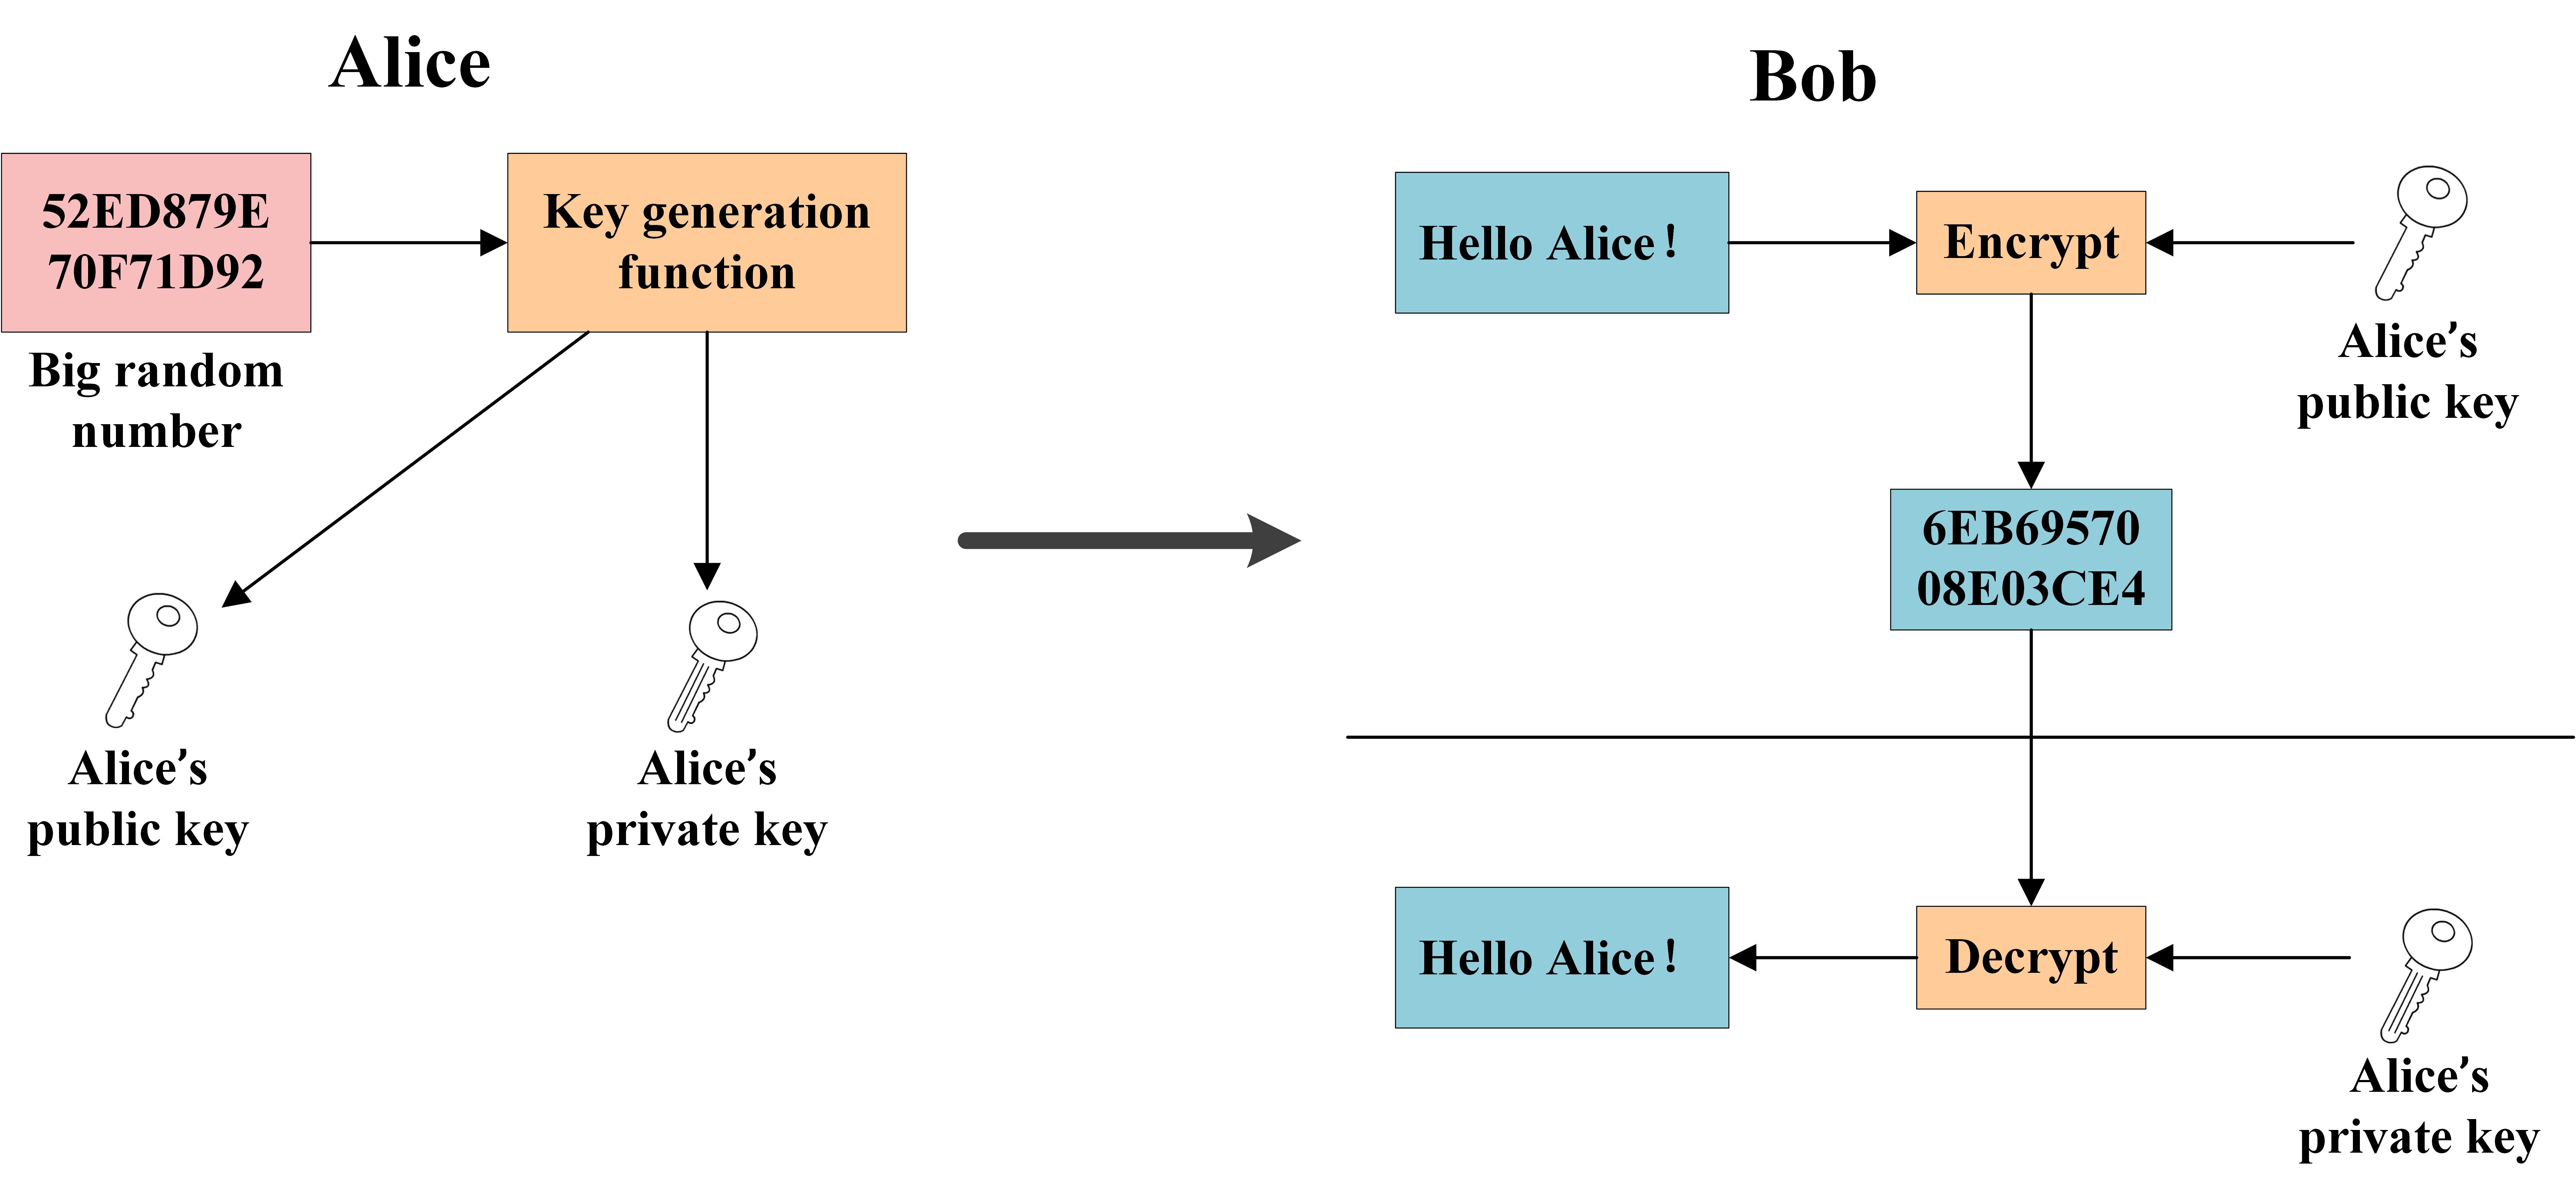
\includegraphics[width=13cm]{figures/pica2.png}
	\caption{典型公钥密码系统}
	\label{pica2}
\end{figure}

在实际使用中,为了平衡对称密码和非对称密码的优缺点,双方之间进行通信通常使用混合加密系统\cite{menezes2018handbook}。首先使用非对称加密在彼此之间达成共享会话密钥(如Diffe-Hellman密钥交换协议),然后使用对称加密传输实际数据。混合加密体制已经安全高效的运行了许多年,但是量子计算的快速发展给以数学问题复杂性为基础的公钥密码体制和以密钥长度为安全基础的对称密码体制带来了灾难性的影响,将使得目前主流的密码体制变得不堪一击\cite{steane1998quantum}。

针对当前密码体制面临的量子计算威胁,近年来美国国家标准与技术研究院(National Institute of Standards and Technology, NIST)已经开始组织设计后量子密码技术(Post-Quantum Cryptography, PQC)\cite{bernstein2009introduction}。后量子密码技术即探索在量子计算条件下的非线性多项式时间可解的 NP 数学问题,典型例子如格基加密算法和基于哈希的加密算法等。无论是经典密码体制,抑或是PQC,其安全性基础都建立在计算资源有限条件下的数学难解问题,无法满足香农提出的信息论安全(Information-theoretical security)级别的信息加密服务。信息论安全通信由信息论安全的密钥分发和信息论安全的加密算法来保证,1949~年,C. E. Shannon 首次系统阐述了消息使用一次一密(One time pad, OTP)算法可以满足无条件安全通信的要求,并指出该算法所使用密钥的熵必须大于等于明文的熵\cite{shannon1949communication}。

物理密码技术的出现打破了传统密码技术的发展瓶颈,并迅速成为国际上信息安全技术的研究热点,以达到信息论防护级别的量子密钥分发(Quantum key distribution, QKD)和物理不可克隆函数(Physical unclonable functions, PUF)为典型代表。量子密钥分发于~1984~年C. H. Bennett和G. Brassard首次提出,基于量子力学的基本特征(不可克隆定理,量子纠缠,测不准原理)为Alice和Bob提供了信息论安全的密钥交换\cite{bb84first,shor2000simple}。因此,Alice和Bob可以基于量子态的传输和测量来共享密钥,而Eve在不引入扰动的情况下无法提取有关密钥的任何信息\cite{gisin2002quantum,liuboliangzi}。量子密钥分发由于其中继转发和经典认证等问题,目前还难以大面积实用化,但是其理论研究和工程实践的成果不仅推动了物理密码的发展,还带来了量子信息领域的变革\cite{xu2020secure,pirandola2020advances,maes2013physically,bennett1992experimental}。物理不可克隆函数最早可追溯至 2001 年 R. Pappu 等人提出的物理单向函数(Physical one-way functions, POF)概念,是一种基于物理、生物微观结构构建 POF 的思想\cite{Pappu2002Physical},并由 B. Gassend 等人实现第一个硅基集成电路 PUF\cite{gassend2002}。PUF 是一种架构在物理实体上的函数关系,挑战响应由其特殊的物理结构决定,并且特定输入对应唯一输出,具备唯一性、稳定性且不可预测,PUF 的不可克隆特性来源于制造(成长)过程中的不可避免的微小偏差\cite{maes2013physically,halak2018physically}。

半导体超晶格密钥分发是基于孪生超晶格 PUF 驱动混沌同步的一种新型信息论安全密钥分发方案,超晶格密钥分发技术是一种物理随机数的异地共享技术拓展。使用孪生超晶格 PUF 物理实体的预分配代替密钥信息的预分配,由器件不可克隆避免了密钥管理中的敏感信息泄露风险;并且,部署完成的孪生超晶格密钥分发设备,能在公开信道中建立密钥分发协议机制,降低密钥部署和更新的成本,以高速、便捷、随遇组网等特点逐渐成为国内研究热点\cite{liu2018secret,wu2020experimental}。


\section{超晶格密钥分发}
\subsection{超晶格研究历史} 
XXXXXXX





\subsection{超晶格物理不可克隆孪生机理}
XXXXXXX


\subsection{基于孪生超晶格的密钥分发方案}

基于超晶格 PUF 的物理不可克隆孪生特性,陈小明等人提出了利用该特性实现点对点密钥分发的构想\cite{chen2020}。超晶格孪生器件在密码学上可以认为是在异地各自运行的同一密钥同一单向函数,且攻击者无法克隆器件也无法建模器件的任意运行过程及结果。因此利用孪生超晶格器件可以安全实现物理随机数的异地排他性共享,即密钥分发\cite{wu2020experimental,xie2021high}。密钥协商的原理架构如图 \ref{pica10} 所示,可简述如下: 
\begin{enumerate}[(1)]
	\item 定义 Alice 为密钥产生(重建)端,Bob 为密钥重建(产生)端,Alice 和 Bob 在常规通信信道上协商激励信号$C$(可以由第三方负责发送,也可由其中一方传给另一方);
	\item Alice 和 Bob 分别在各自的超晶格 PUF 中输入$C$得到原始输出数据,对原始输出进行高精准离线序列同步得到响应$W$和$W'$,$W$和$W'$汉明距离大约为 10\% ;
	\item Alice 计算辅助数据$H$,并将$H$通过公开信道传送给 Bob,Bob 在$H$的帮助下和$W'$计算出$W$,此过程即为信息调同(Information reconciliation)\cite{dodis2004fuzzy};
	\item Alice、Bob 双方根据$H$泄露的信息和器件输出的极小熵,从$W$中提取出相同密钥$R$,此过程即为保密增强(Privacy amplification, PA)\cite{bennett1995generalized}。
\end{enumerate}


\begin{figure}[h]
	\centering
	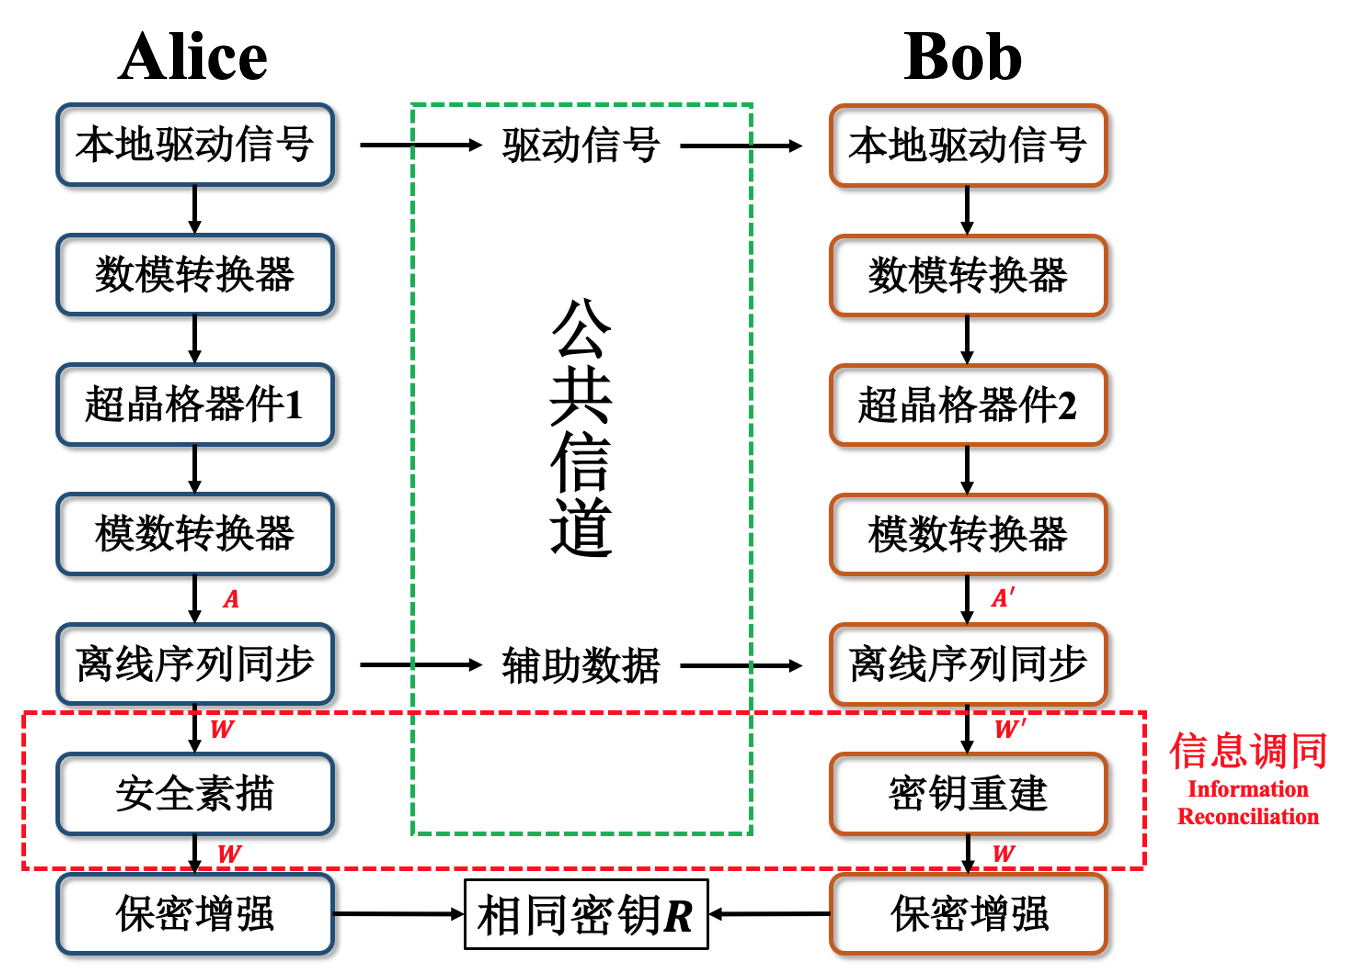
\includegraphics[width=13cm]{pica10.png}
	\caption{基于超晶格PUF的密钥分发协议}
	\label{pica10}
\end{figure}

信息调同用来描述从$W'$恢复出$W$的过程,此过程不会泄漏很多关于$W$的信息,一般用安全素描实现。保密增强的一般实现方案为一致哈希函数(Universal hash functions, UHF)提取器实现\cite{carter1979universal},该函数的输入为非满熵的待提取的随机数和公开的满熵随机数,输出保密的满熵随机数。信息调同和保密增强统称模糊提取器(Fuzzy extractor),可以从物理、生物等唯一特征数据中提取出可用作加密、认证的密钥。


\section{论文主要工作与结构安排}
\subsection{主要工作}

本文的主要研究内容是超晶格密钥分发系统的后处理部分,研究面向实际应用的高精准序列同步算法、高吞吐率的信息调同算法、无条件安全保密增强算法,并开展了相关实验验证。本文对超晶格密钥分发系统的高速高效后处理算法进行了深入研究,取得的主要创新工作如下:

\begin{enumerate}[(1)]
	\item 研究超晶格密钥分发过程中通信双方的高精准序列同步技术。XXXXXXX
	\item 研究高吞吐率的信息调同技术。XXXXXXX
	\item 研究超晶格密钥分发无条件安全保密增强技术。XXXXXXX
	\item 超晶格密钥分发系统安全密钥分发实验。XXXXXXX
\end{enumerate}

\subsection{结构安排}

本文结构组织如下:

第\ref{ch1}章,绪论,即本章。从现代密码学中的密钥管理问题介绍了现今物理密码体系的发展和突破,进而引出超晶格密钥分发技术,介绍了超晶格密钥分发系统后处理技术的研究背景、意义以及本文的主要研究内容。

第\ref{ch2}章,超晶格密钥分发后处理技术基础,主要介绍XX。

第\ref{ch3}章,高精准序列同步技术研究。XXXXXXX。

第\ref{ch4}章,高吞吐率的信息调同算法研究。XXXXXXX

第\ref{ch5}章,信息论安全的保密增强算法研究。XXXXXXX

第\ref{ch6}章,异地实时超晶格密钥分发实验。XXXXXXX

第\ref{ch7}章,总结与展望。对全文工作进行总结,并对未来研究作出展望。

